% Supplementary Information for the ChromDecode-At manuscript.
% Figures are read from ../figures/; tables are the CSVs in ../supplementary_tables/
% (indexed in ../supplementary_tables/README.md), so they are listed here, not typeset.

\documentclass[11pt,a4paper]{article}
\usepackage[utf8]{inputenc}
\usepackage{lmodern}
\usepackage[T1]{fontenc}
\usepackage[margin=2.2cm]{geometry}
\usepackage{graphicx}
\usepackage{subcaption}
\usepackage{caption}
\usepackage[hidelinks]{hyperref}
\captionsetup{font=small,labelfont=bf}
\graphicspath{{../figures/}}
\renewcommand{\thefigure}{S\arabic{figure}}

\title{\bfseries Supplementary Information\\[2pt]\large Expression-to-chromatin decoding of the
\textit{Arabidopsis} spaceflight transcriptome}
\author{Richard J. Barker}
\date{}

\begin{document}
\maketitle

\section*{Supplementary tables}
Tables S1--S57 and D1--D7 are CSV files in \texttt{supplementary\_tables/} and \texttt{data/derived/} of the
archive. The index there (\texttt{supplementary\_tables/README.md}) gives, for each table, its content, the
script that writes it, the manuscript section that cites it, and the audit notes on how to read it.

\section*{Supplementary figures}

\begin{figure}[h]
\centering
\begin{subfigure}{0.32\textwidth}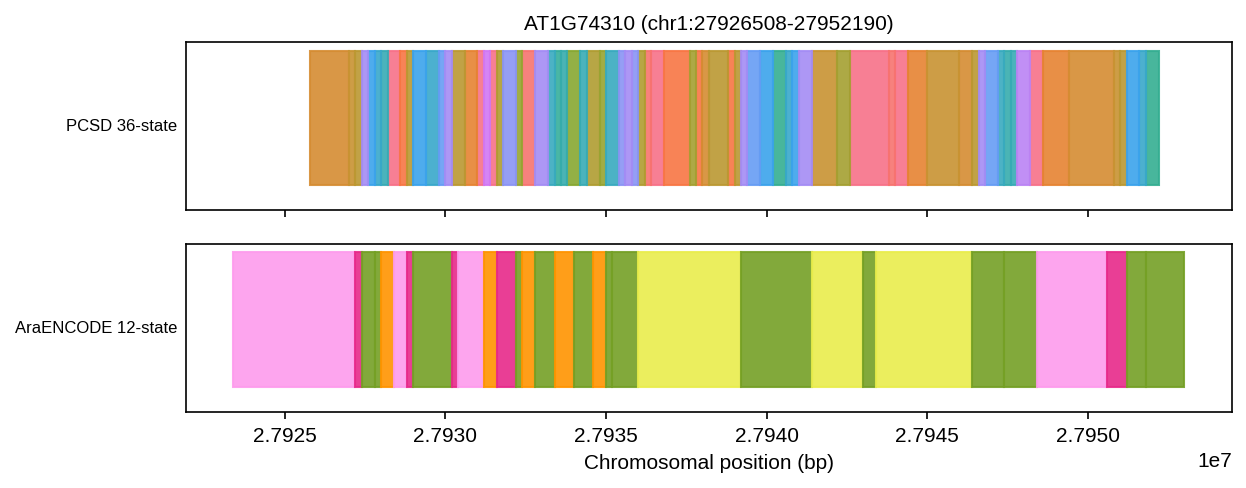
\includegraphics[width=\linewidth]{fig4_locus_AT1G74310.png}\caption{}\end{subfigure}
\begin{subfigure}{0.32\textwidth}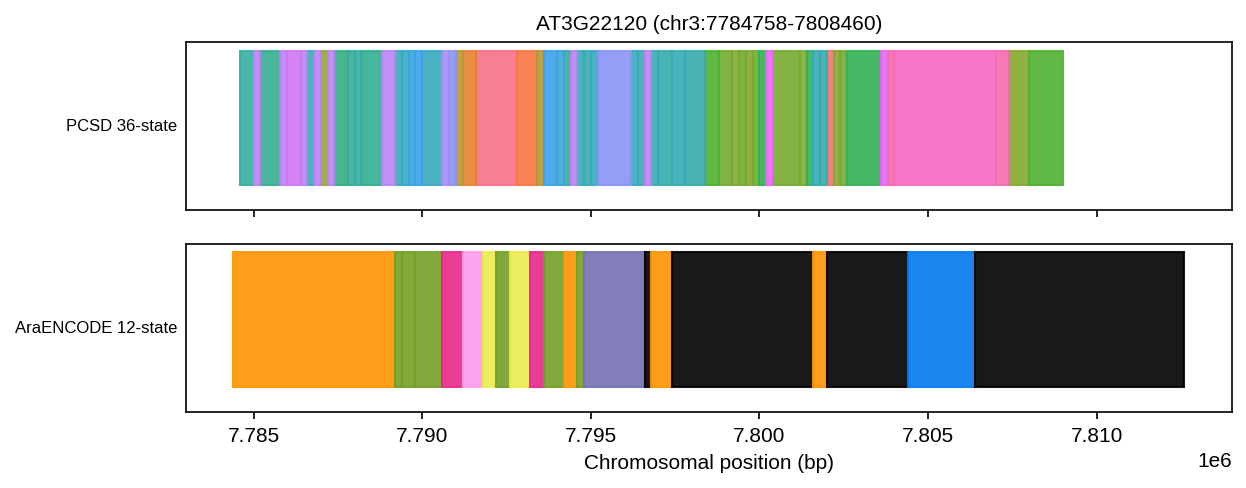
\includegraphics[width=\linewidth]{fig4_locus_AT3G22120.png}\caption{}\end{subfigure}
\begin{subfigure}{0.32\textwidth}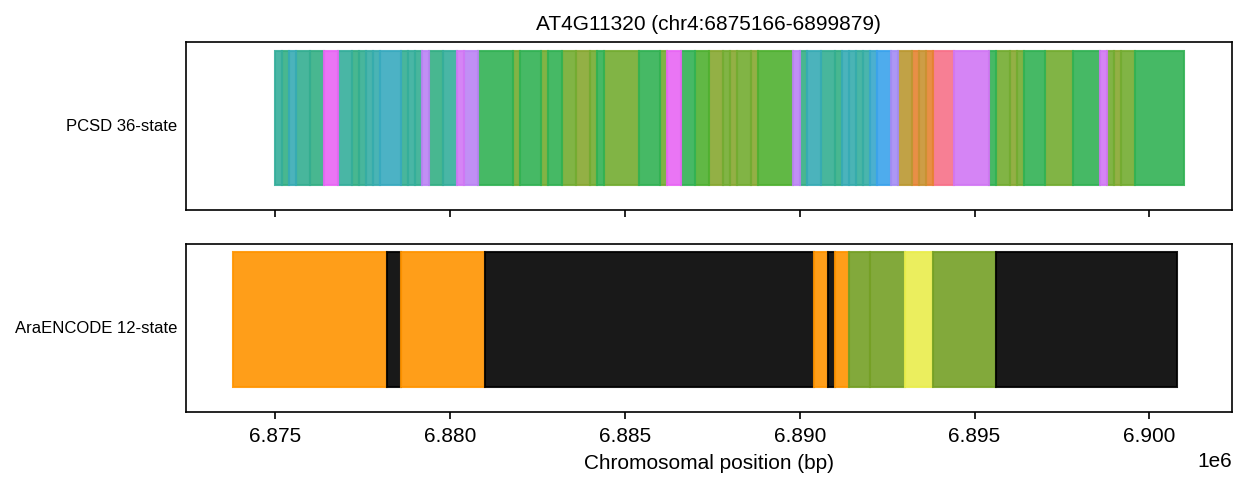
\includegraphics[width=\linewidth]{fig4_locus_AT4G11320.png}\caption{}\end{subfigure}
\caption{Locus views of three OSD-37 differentially expressed genes, showing PCSD 36-state and AraENCODE 12-state
tracks across the gene body and 2\,kb upstream (v1).}
\end{figure}

\begin{figure}[h]\centering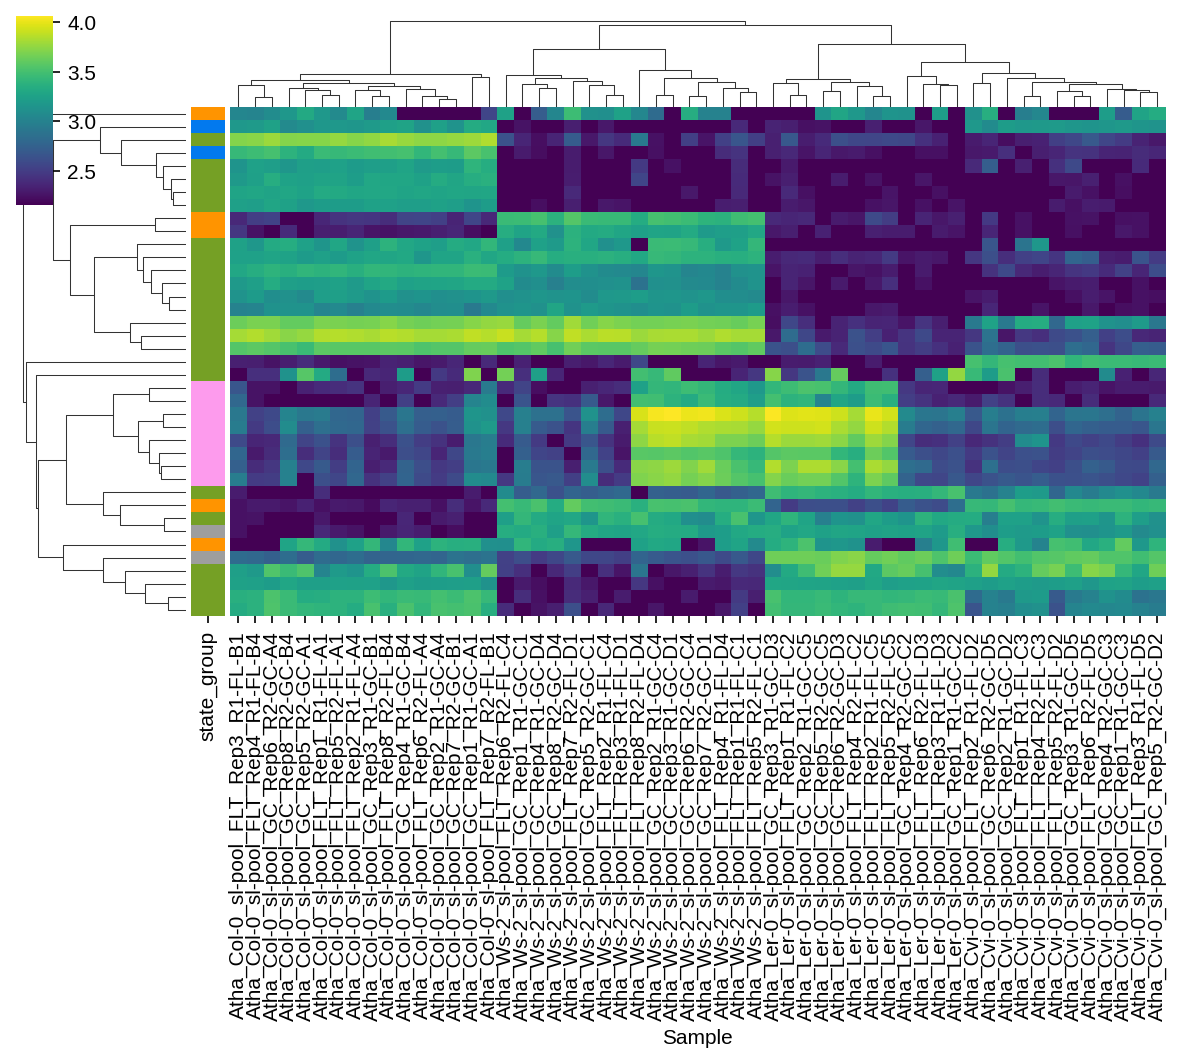
\includegraphics[width=0.8\textwidth]{fig5_heatmap_topDEGs.png}
\caption{Expression of the top OSD-37 DEGs across samples, annotated by chromatin-state group (v1).}\end{figure}

\begin{figure}[h]\centering
\begin{subfigure}{0.48\textwidth}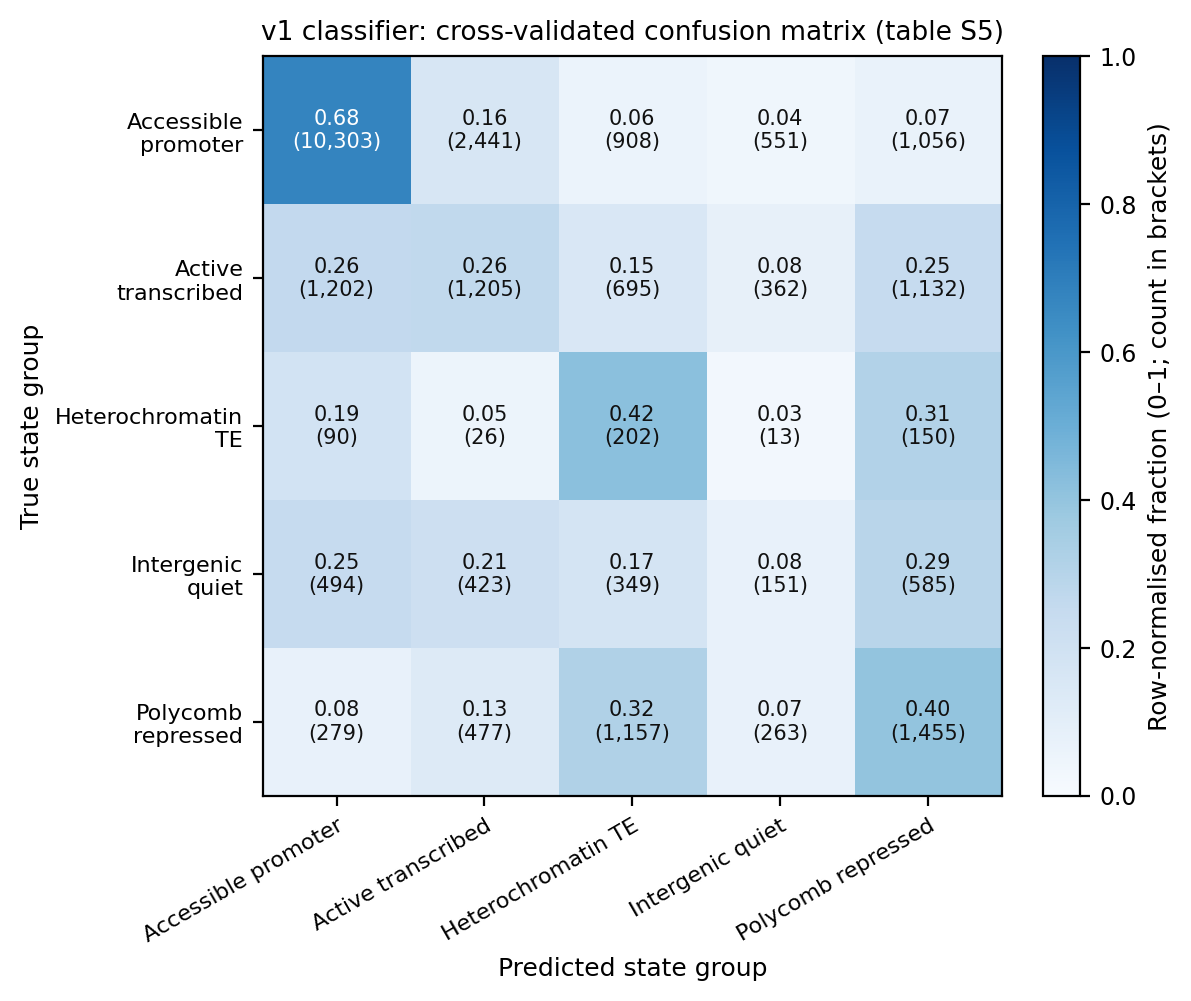
\includegraphics[width=\linewidth]{fig6_confusion_matrix.png}\caption{}\end{subfigure}
\begin{subfigure}{0.48\textwidth}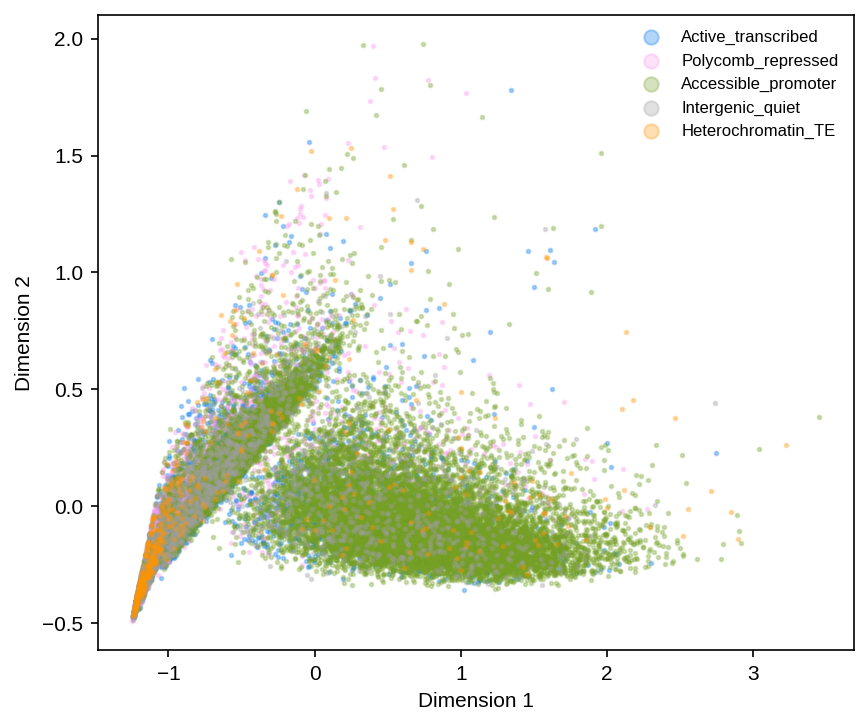
\includegraphics[width=\linewidth]{fig7_state_space_projection.png}\caption{}\end{subfigure}
\caption{v1 learned layer. (a) Cross-validated confusion matrix (Table~S5). (b) Projection of genes in
expression-feature space, coloured by chromatin-state group.}\end{figure}

\begin{figure}[h]\centering
\begin{subfigure}{0.48\textwidth}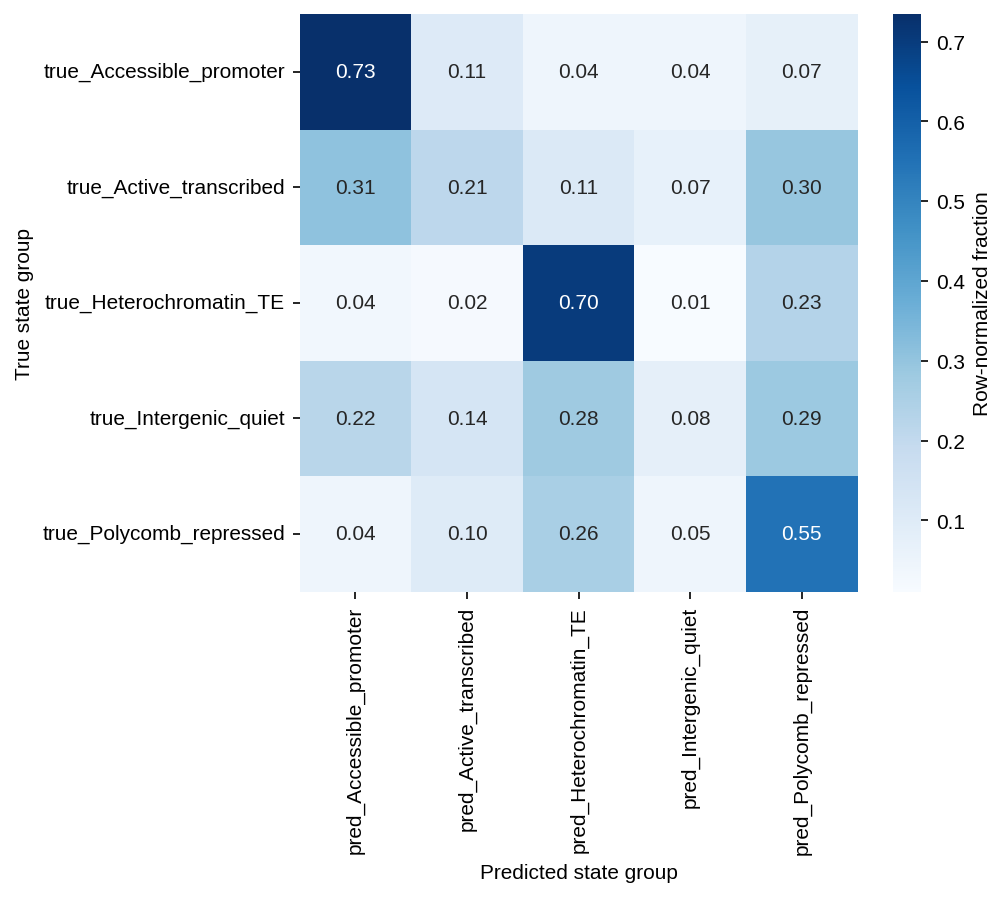
\includegraphics[width=\linewidth]{fig8_v2_confusion_matrix.png}\caption{}\end{subfigure}
\begin{subfigure}{0.48\textwidth}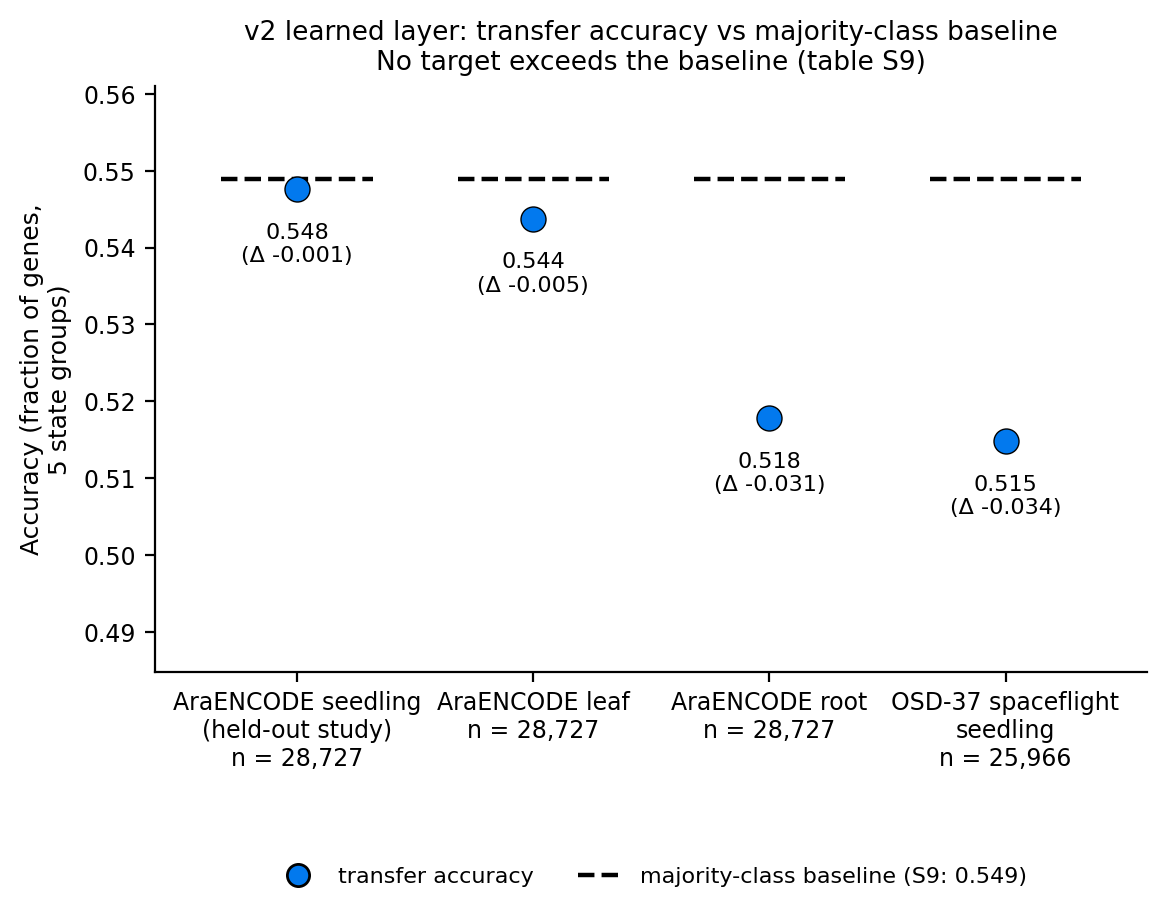
\includegraphics[width=\linewidth]{fig9_v2_transfer.png}\caption{}\end{subfigure}
\caption{v2 learned layer (tissue-matched AraENCODE training). (a) Confusion matrix (Table~S8). (b) Transfer
accuracy against the majority-class baseline (Table~S9); no transfer exceeds the baseline.}\end{figure}

\begin{figure}[h]\centering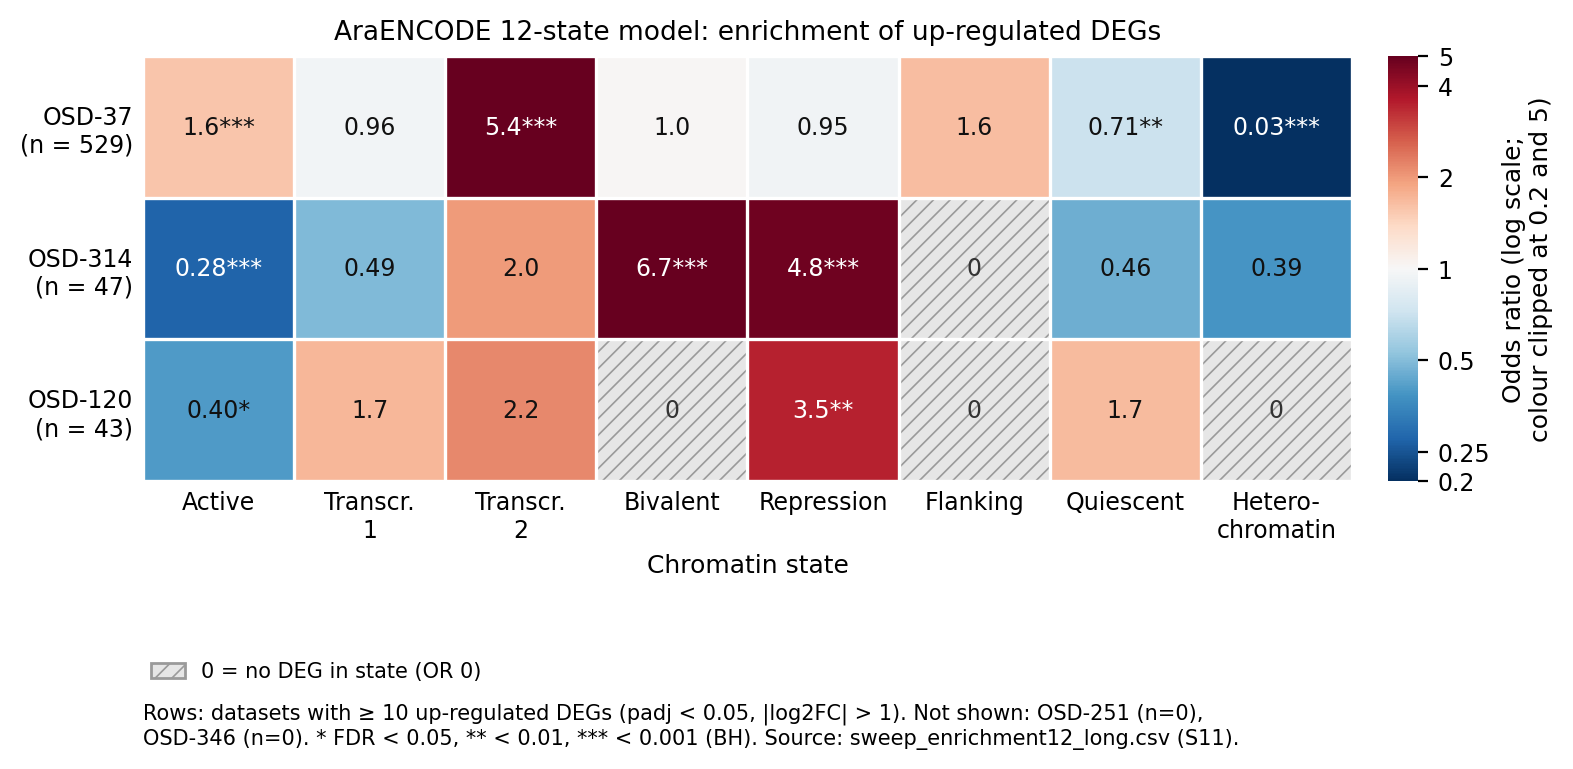
\includegraphics[width=0.85\textwidth]{fig13_sweep_heatmap_12state_up.png}
\caption{AraENCODE 12-state enrichment of up-regulated DEGs across OSDR datasets (Table~S11).}\end{figure}

\begin{figure}[h]\centering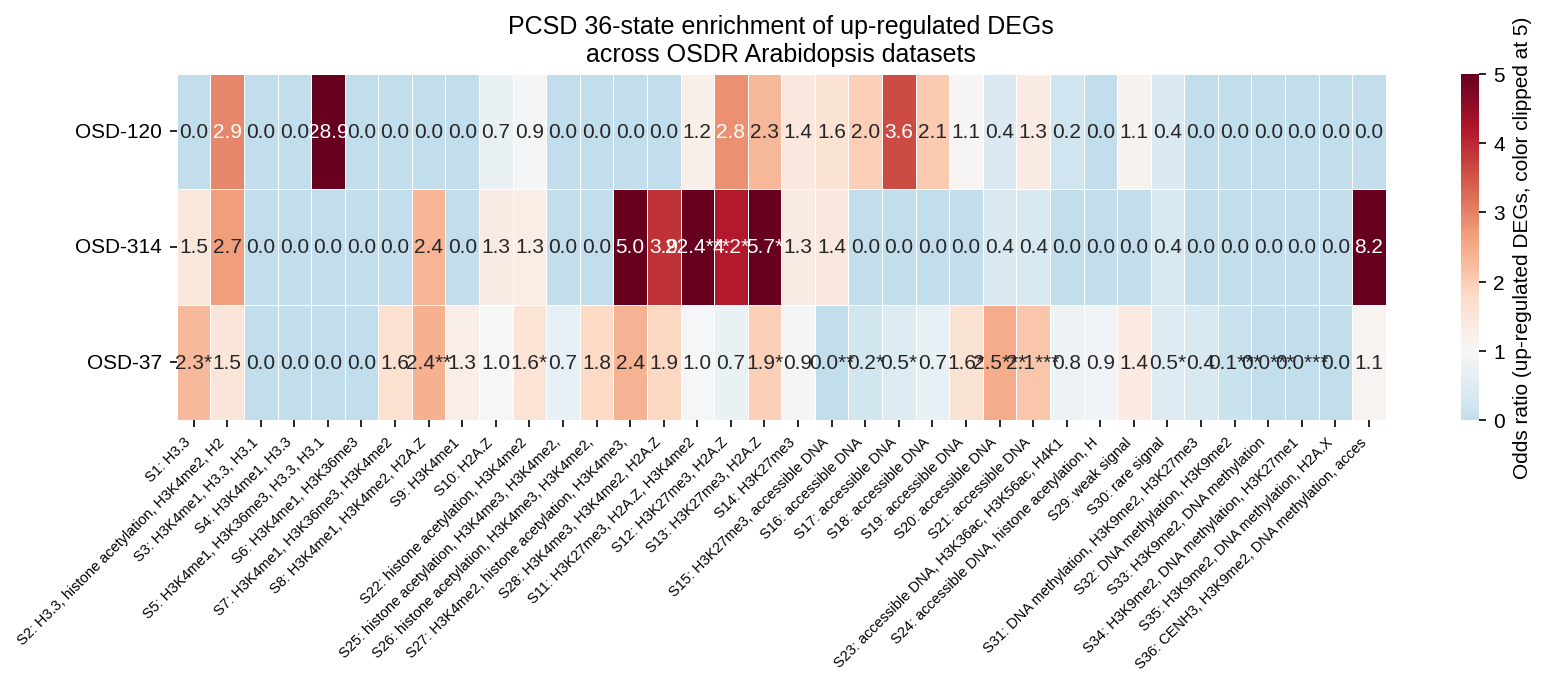
\includegraphics[width=\textwidth,height=0.8\textheight,keepaspectratio]{fig15_sweep_heatmap_36state_up.png}
\caption{PCSD 36-state enrichment of up-regulated DEGs across OSDR datasets (Table~S12). The OSD-314 row uses the
published pooled contrast; corrected values are in main-text Figs.~3 and 7.}\end{figure}

\begin{figure}[h]\centering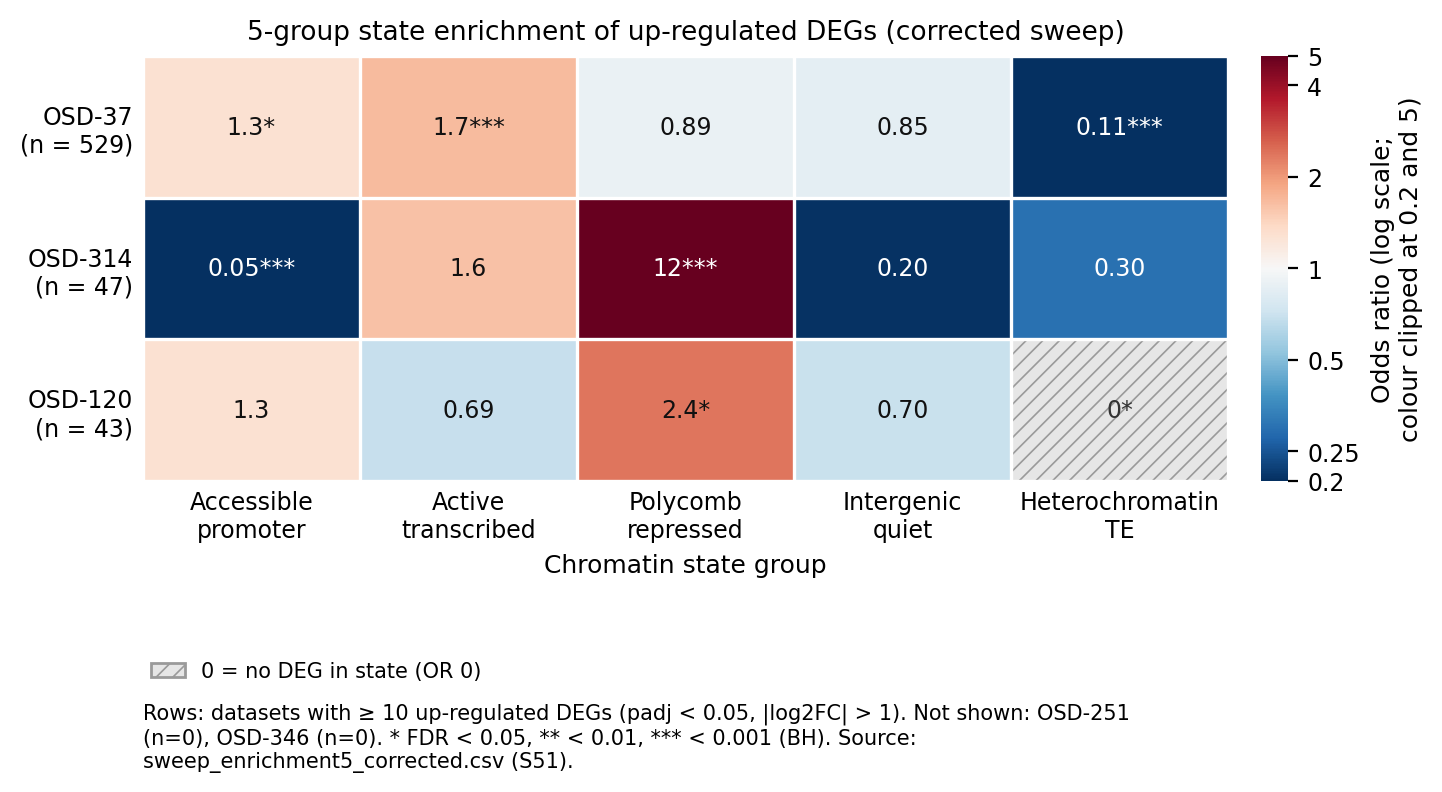
\includegraphics[width=0.75\textwidth]{fig10_sweep_heatmap_up.png}
\caption{5-group state enrichment of up-regulated DEGs across OSDR datasets (corrected sweep, Table~S51).}\end{figure}

\begin{figure}[h]\centering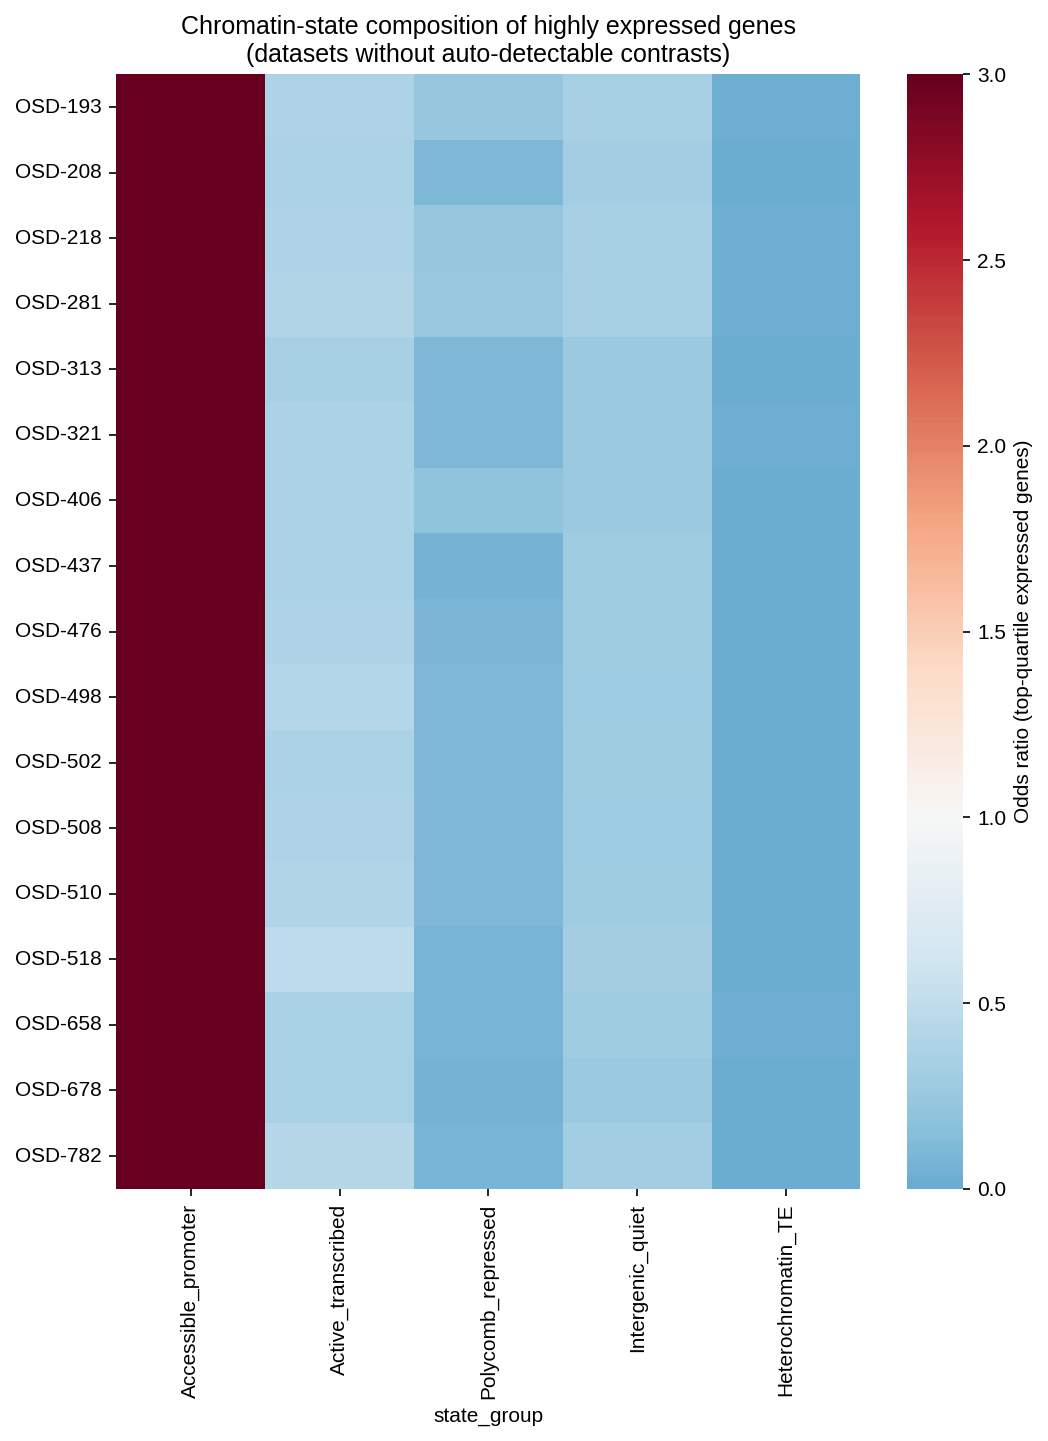
\includegraphics[width=0.75\textwidth]{fig11_sweep_heatmap_expr_only.png}
\caption{Expression-only fallback decoding across the 18 datasets without a detectable contrast: highly expressed
genes sit in accessible-promoter chromatin in every dataset, so the panel is a sanity check and carries no
condition-specific signal (Table~S10).}\end{figure}

\begin{figure}[h]\centering
\begin{subfigure}{0.48\textwidth}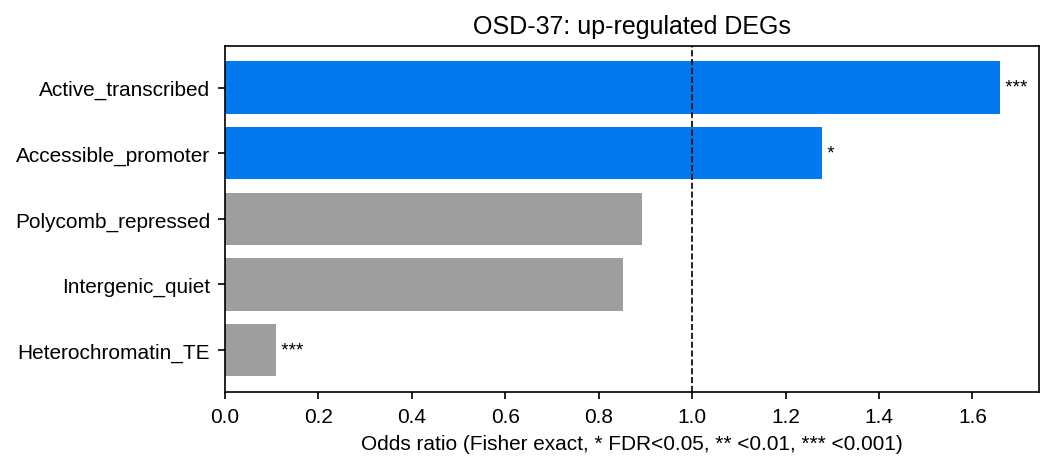
\includegraphics[width=\linewidth]{fig12_OSD-37_enrichment_up.png}\caption{}\end{subfigure}
\begin{subfigure}{0.48\textwidth}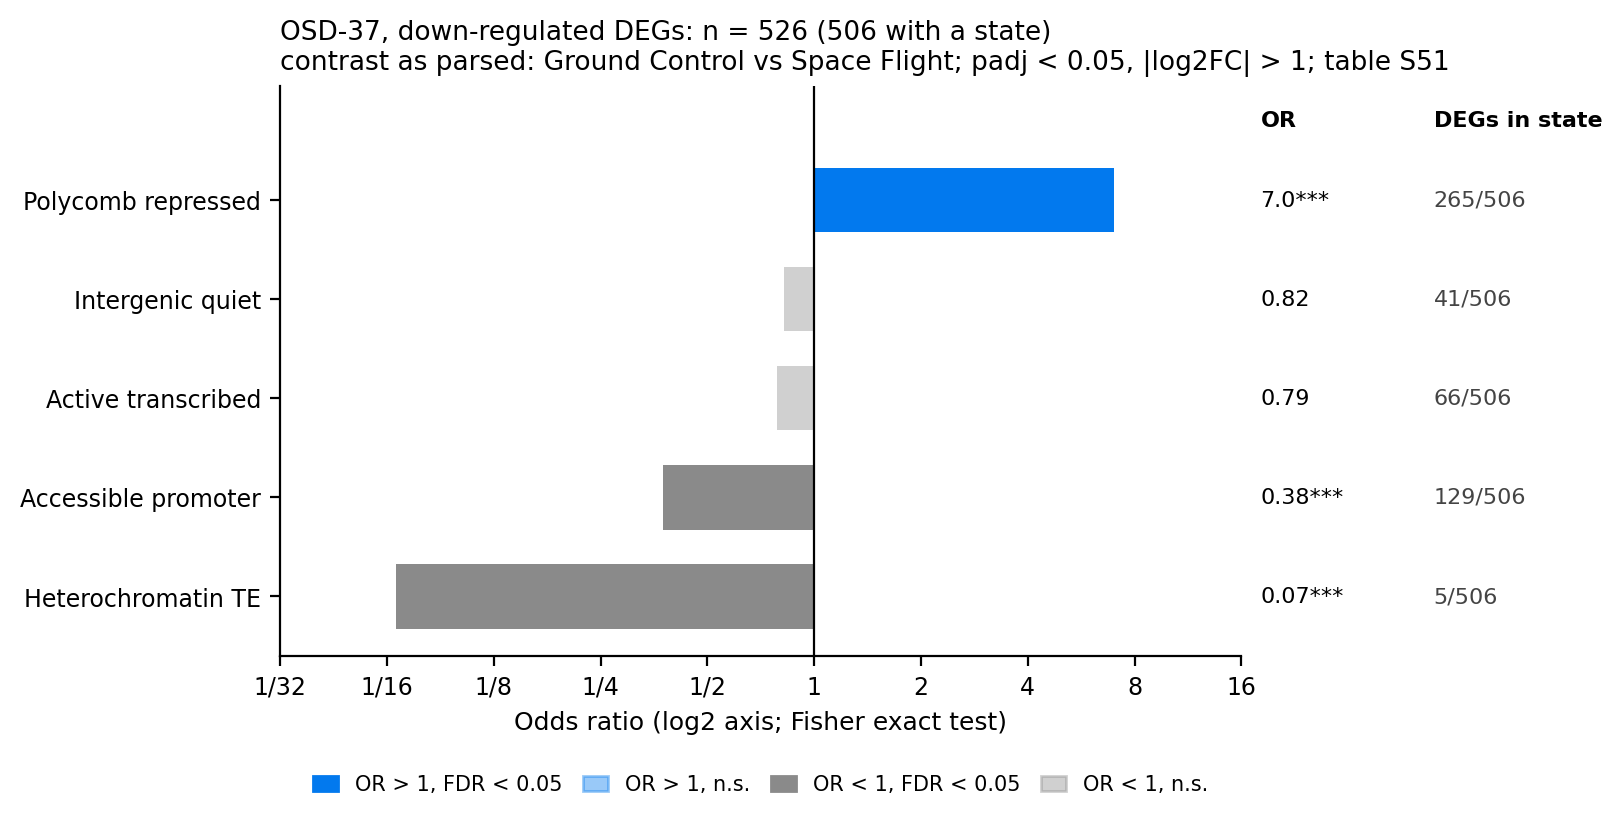
\includegraphics[width=\linewidth]{fig12_OSD-37_enrichment_down.png}\caption{}\end{subfigure}\\
\begin{subfigure}{0.48\textwidth}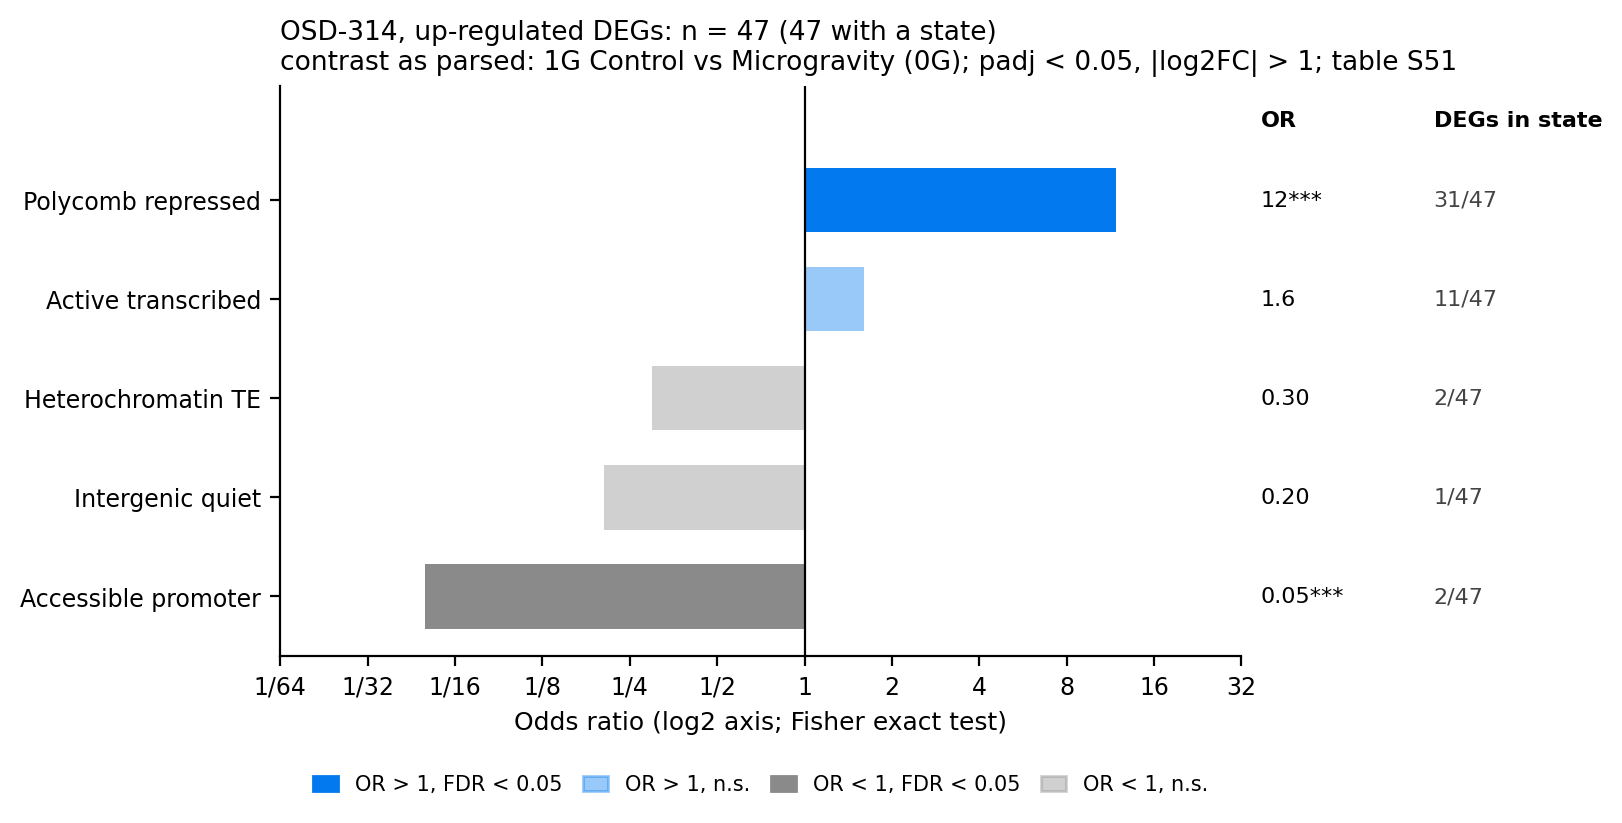
\includegraphics[width=\linewidth]{fig12_OSD-314_enrichment_up.png}\caption{}\end{subfigure}
\begin{subfigure}{0.48\textwidth}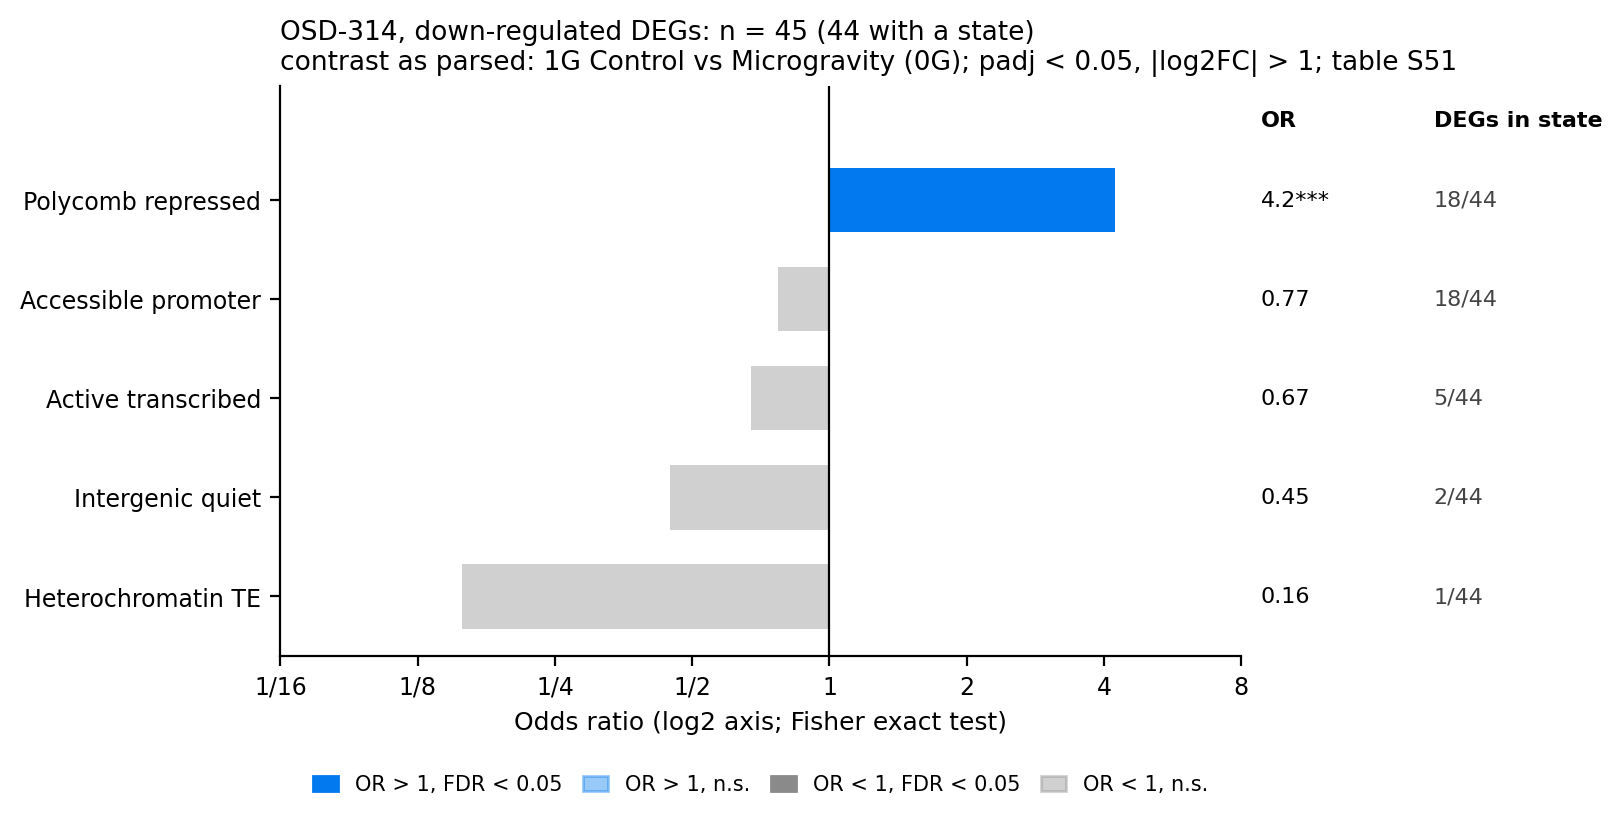
\includegraphics[width=\linewidth]{fig12_OSD-314_enrichment_down.png}\caption{}\end{subfigure}\\
\begin{subfigure}{0.48\textwidth}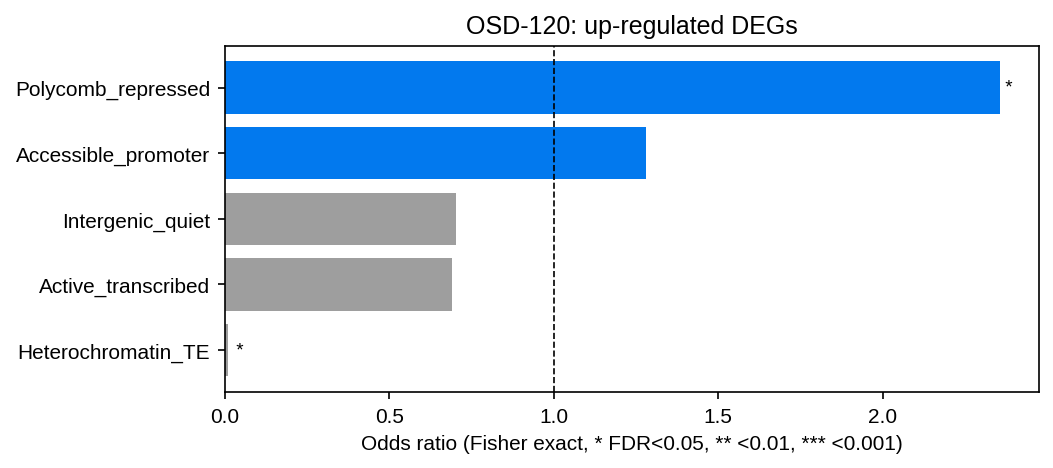
\includegraphics[width=\linewidth]{fig12_OSD-120_enrichment_up.png}\caption{}\end{subfigure}
\begin{subfigure}{0.48\textwidth}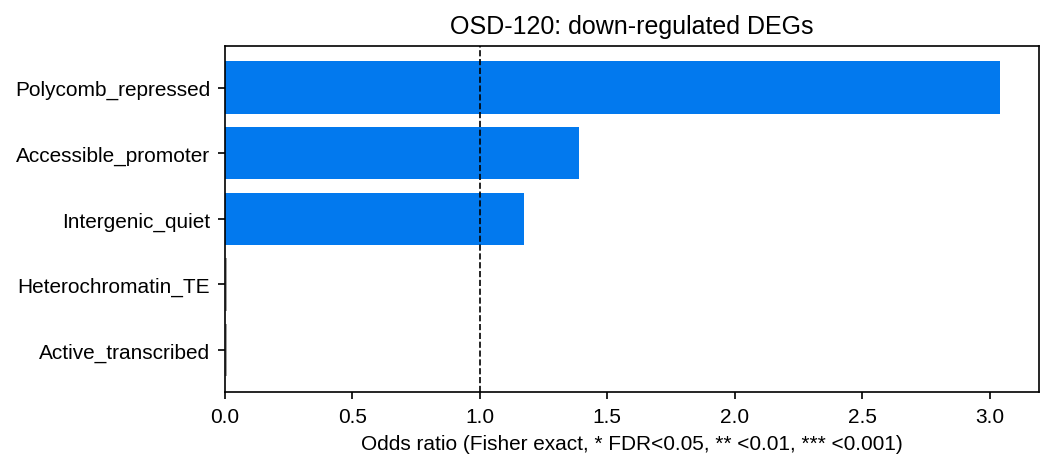
\includegraphics[width=\linewidth]{fig12_OSD-120_enrichment_down.png}\caption{}\end{subfigure}
\caption{Per-dataset 5-group enrichment of up- and down-regulated DEGs: (a, b) OSD-37, (c, d) OSD-314 (published
pooled contrast), (e, f) OSD-120 (mixed genotypes). OSD-251 and OSD-346 have at most one DEG and are not estimable
(Table~S51).}\end{figure}

\begin{figure}[h]\centering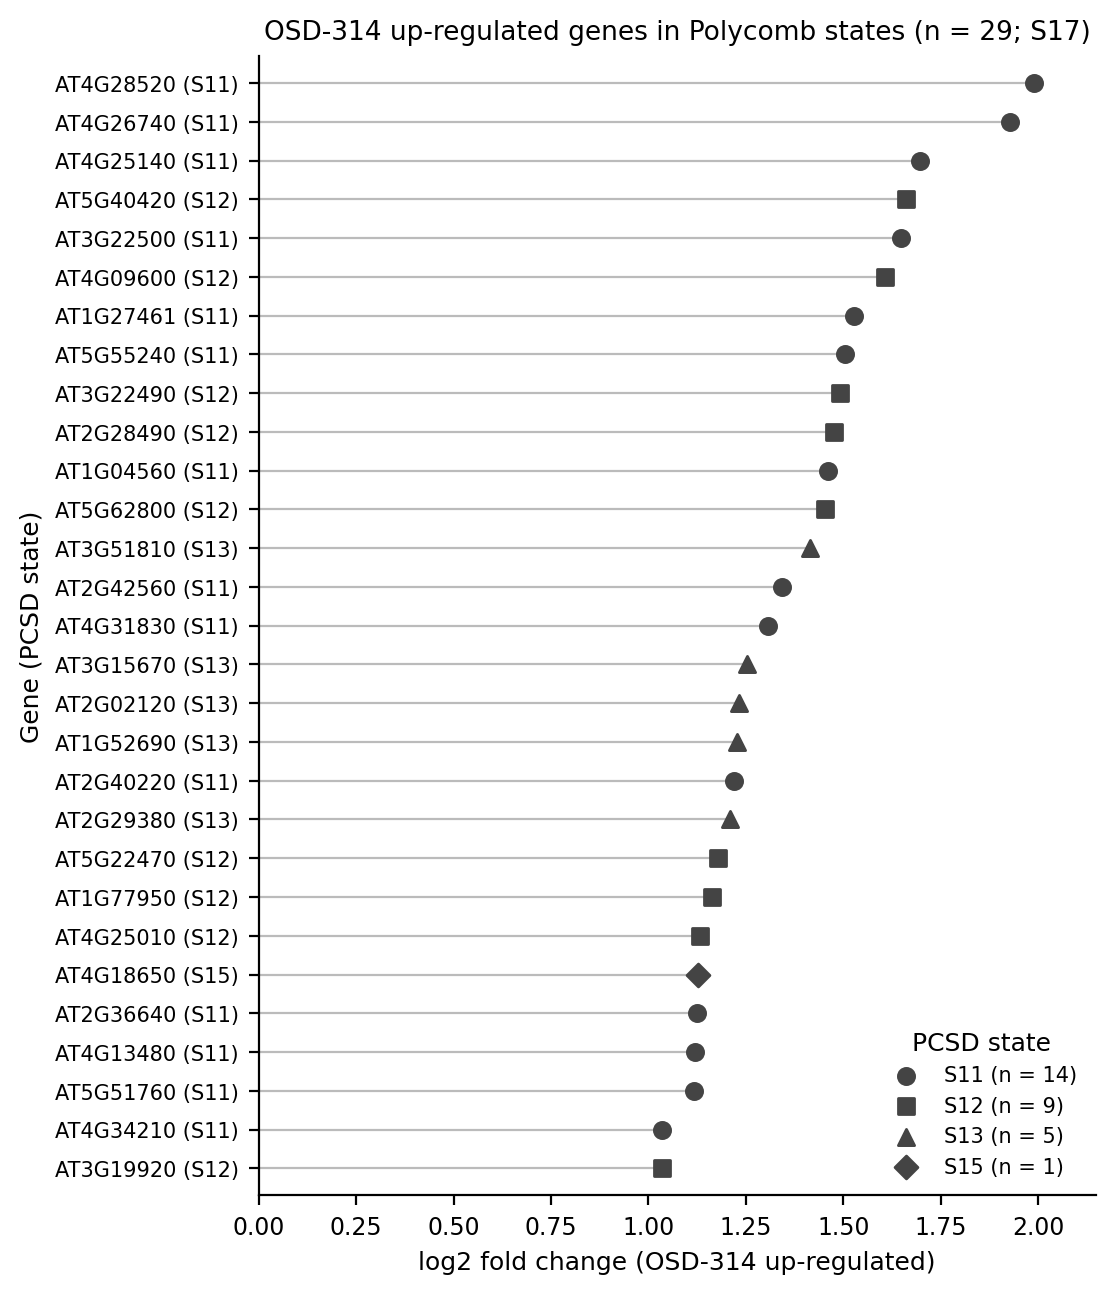
\includegraphics[width=0.75\textwidth]{fig21_polycomb_up_genes.png}
\caption{The 29 OSD-314 up-regulated genes in Polycomb states, in the published pooled contrast (Table~S17). The corrected
contrasts give 255 (0.3\,g) and 302 (0\,g) such genes (Table~S62).}\end{figure}

\begin{figure}[h]\centering
\begin{subfigure}{0.48\textwidth}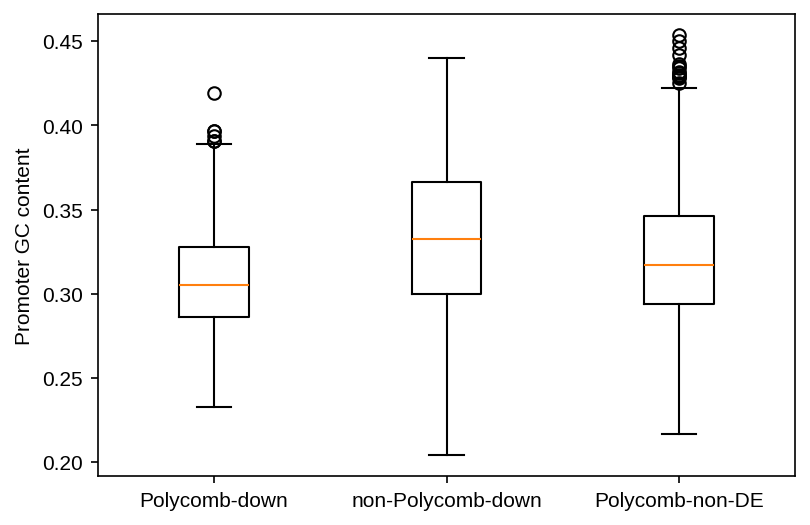
\includegraphics[width=\linewidth]{fig24_gc_content.png}\caption{}\end{subfigure}
\begin{subfigure}{0.48\textwidth}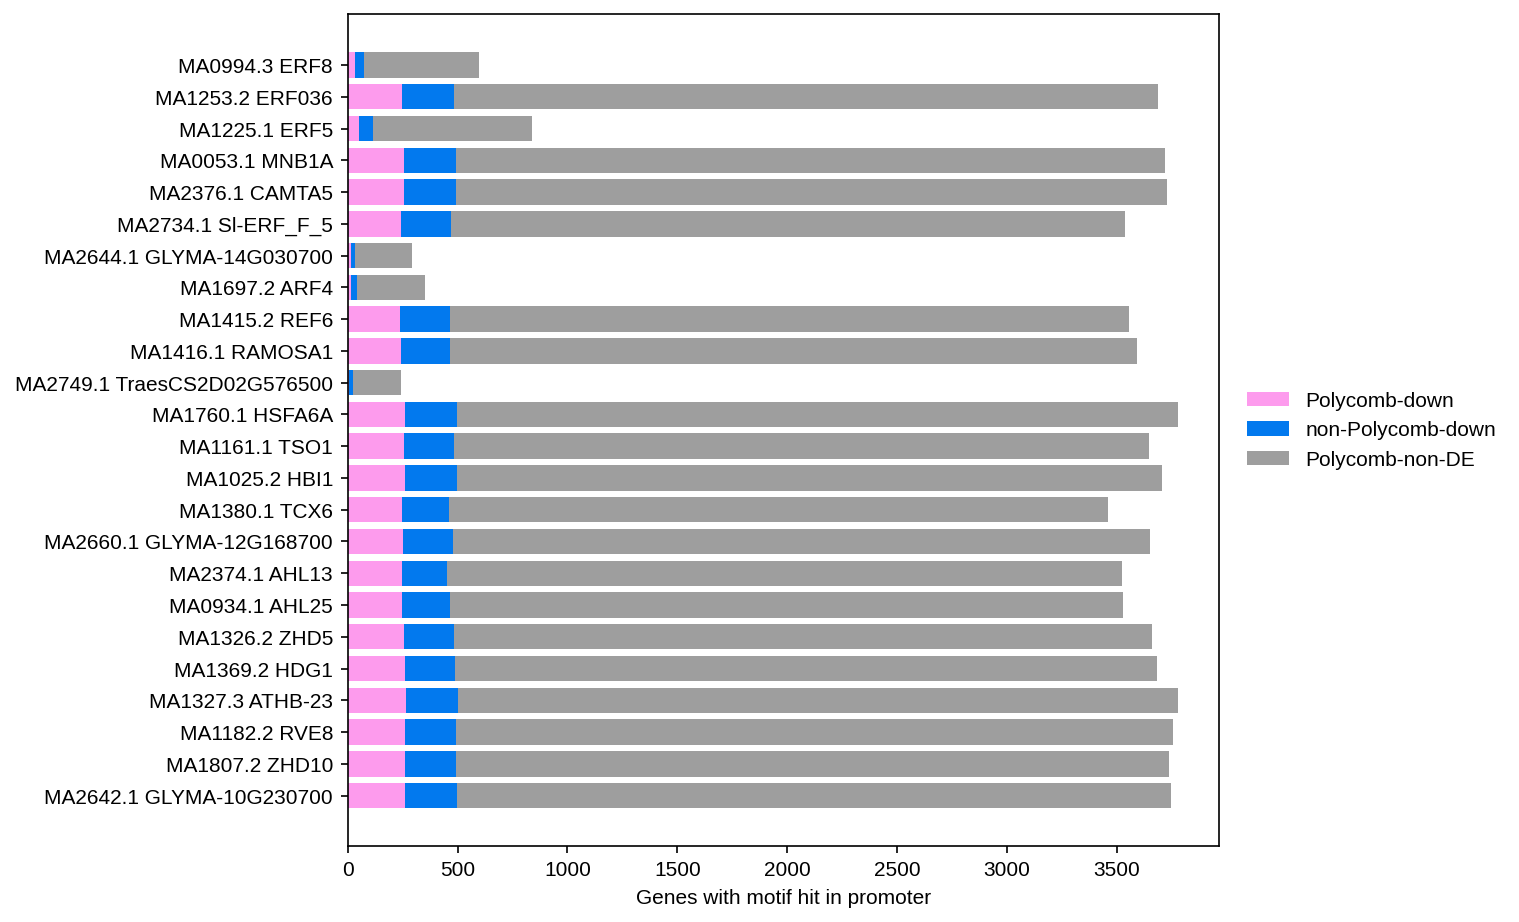
\includegraphics[width=\linewidth]{fig25_motif_overlap.png}\caption{}\end{subfigure}
\caption{Motif-analysis controls. (a) Mean promoter GC content per gene set (Table~S20). (b) Overlap of top-motif
hits among Polycomb-down promoters.}\end{figure}

\begin{figure}[h]\centering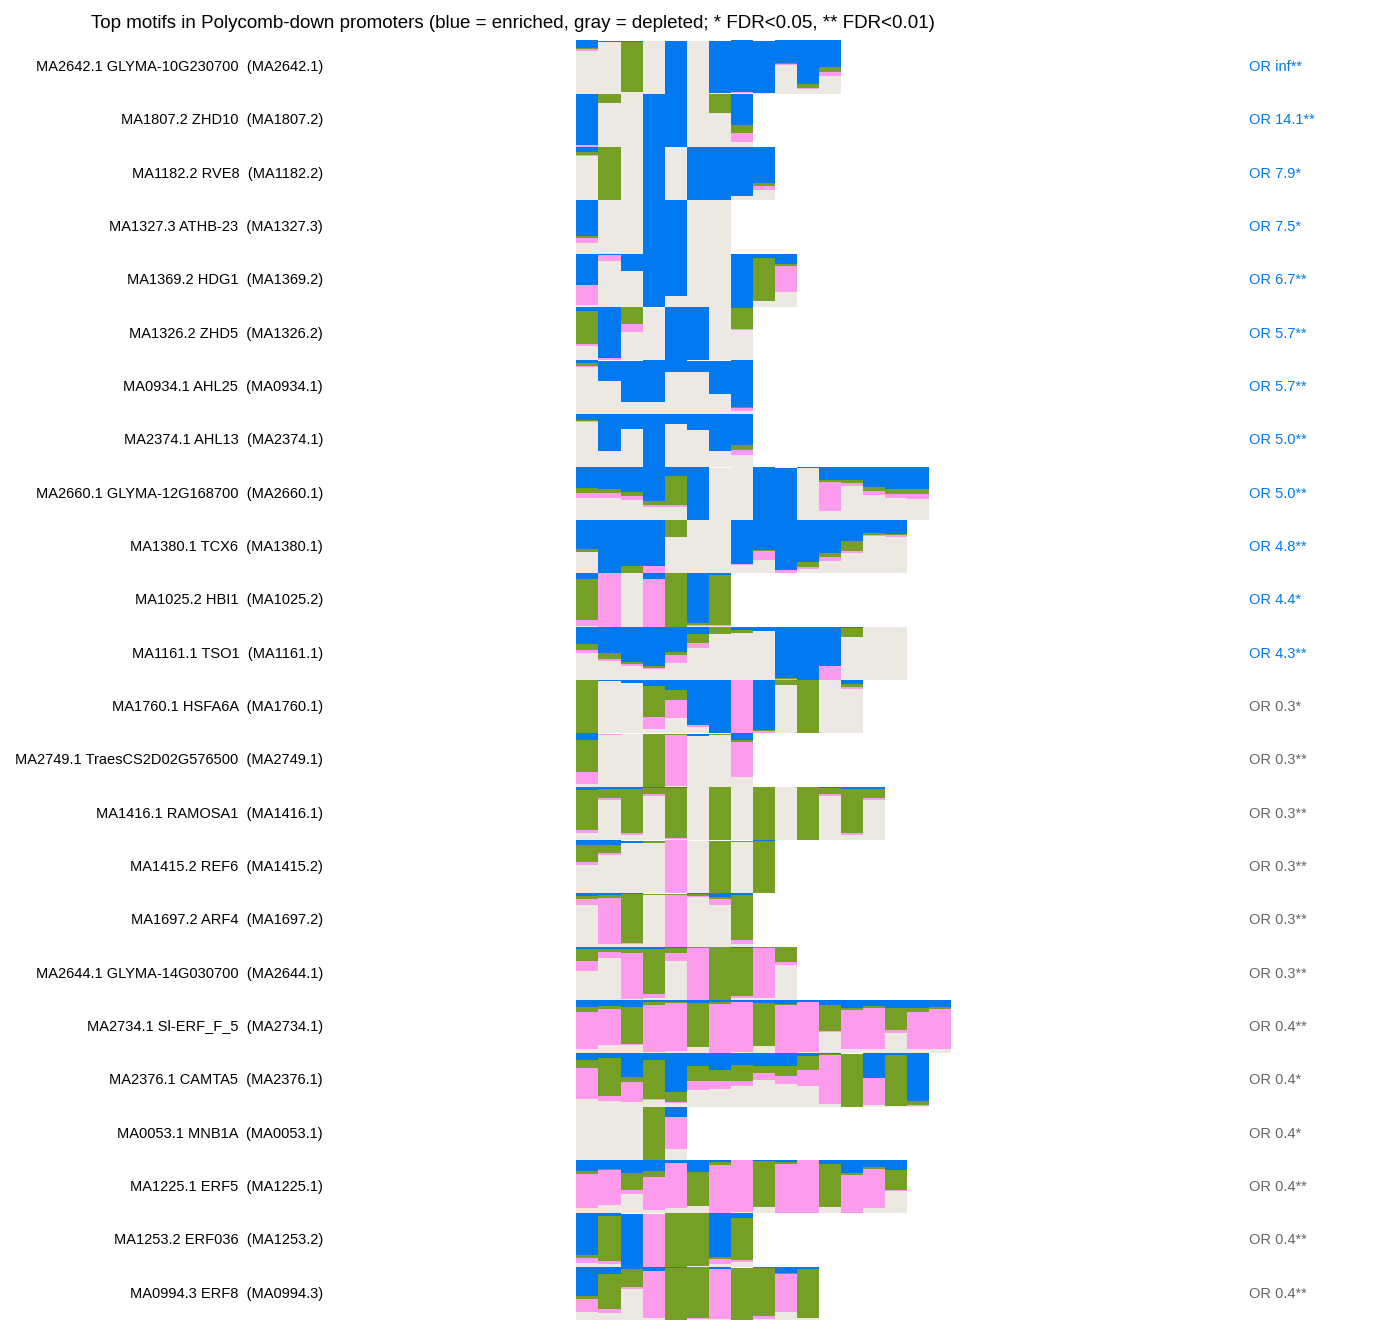
\includegraphics[width=0.85\textwidth]{fig26_motif_logos.png}
\caption{The 12 most enriched and 12 most depleted JASPAR motifs in Polycomb-down promoters (Table~S18).}\end{figure}

\begin{figure}[h]\centering
\begin{subfigure}{0.48\textwidth}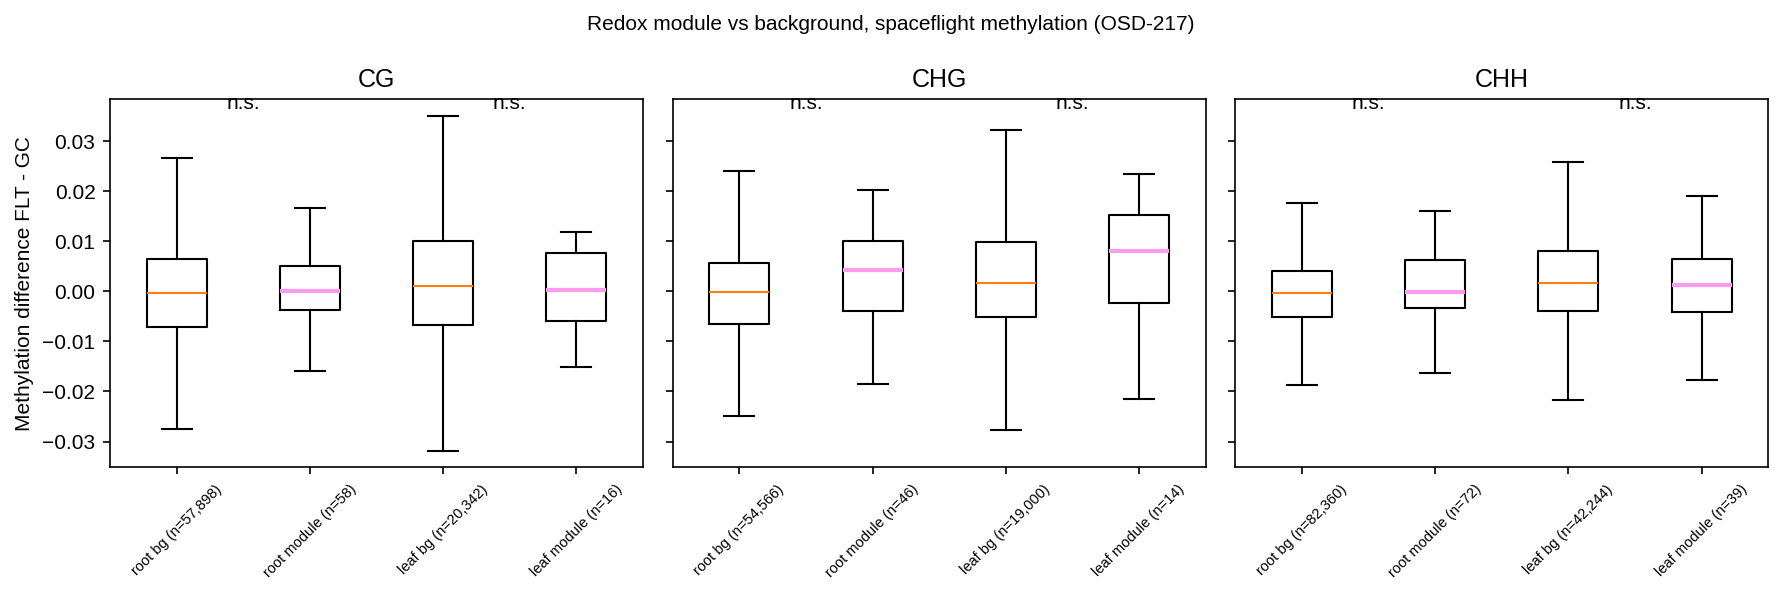
\includegraphics[width=\linewidth]{fig28_methylation_module.png}\caption{}\end{subfigure}
\begin{subfigure}{0.48\textwidth}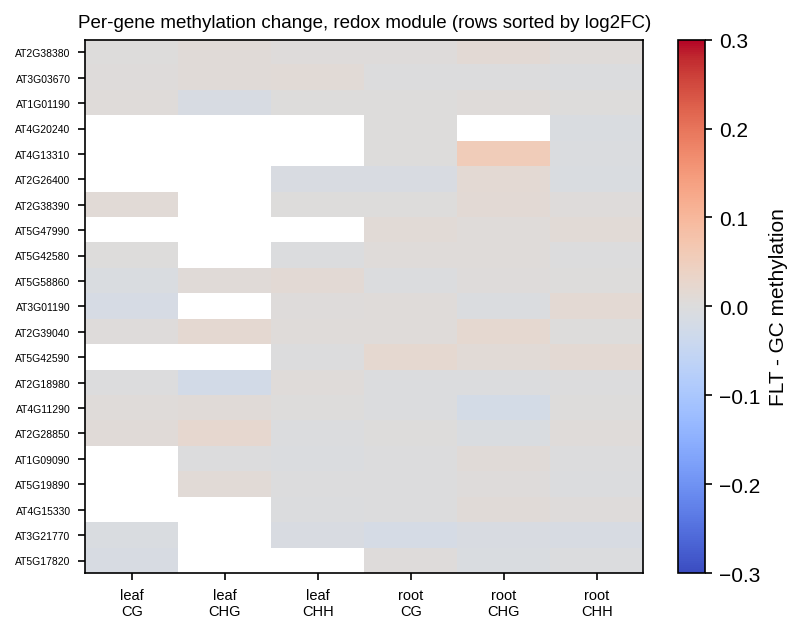
\includegraphics[width=\linewidth]{fig29_methylation_heatmap.png}\caption{}\end{subfigure}
\caption{OSD-217 gene-body methylation, flight minus ground, for the redox module vs background (Table~S22).
(a) Distributions per tissue and context. (b) Per-gene values.}\end{figure}

\begin{figure}[h]\centering
\begin{subfigure}{0.48\textwidth}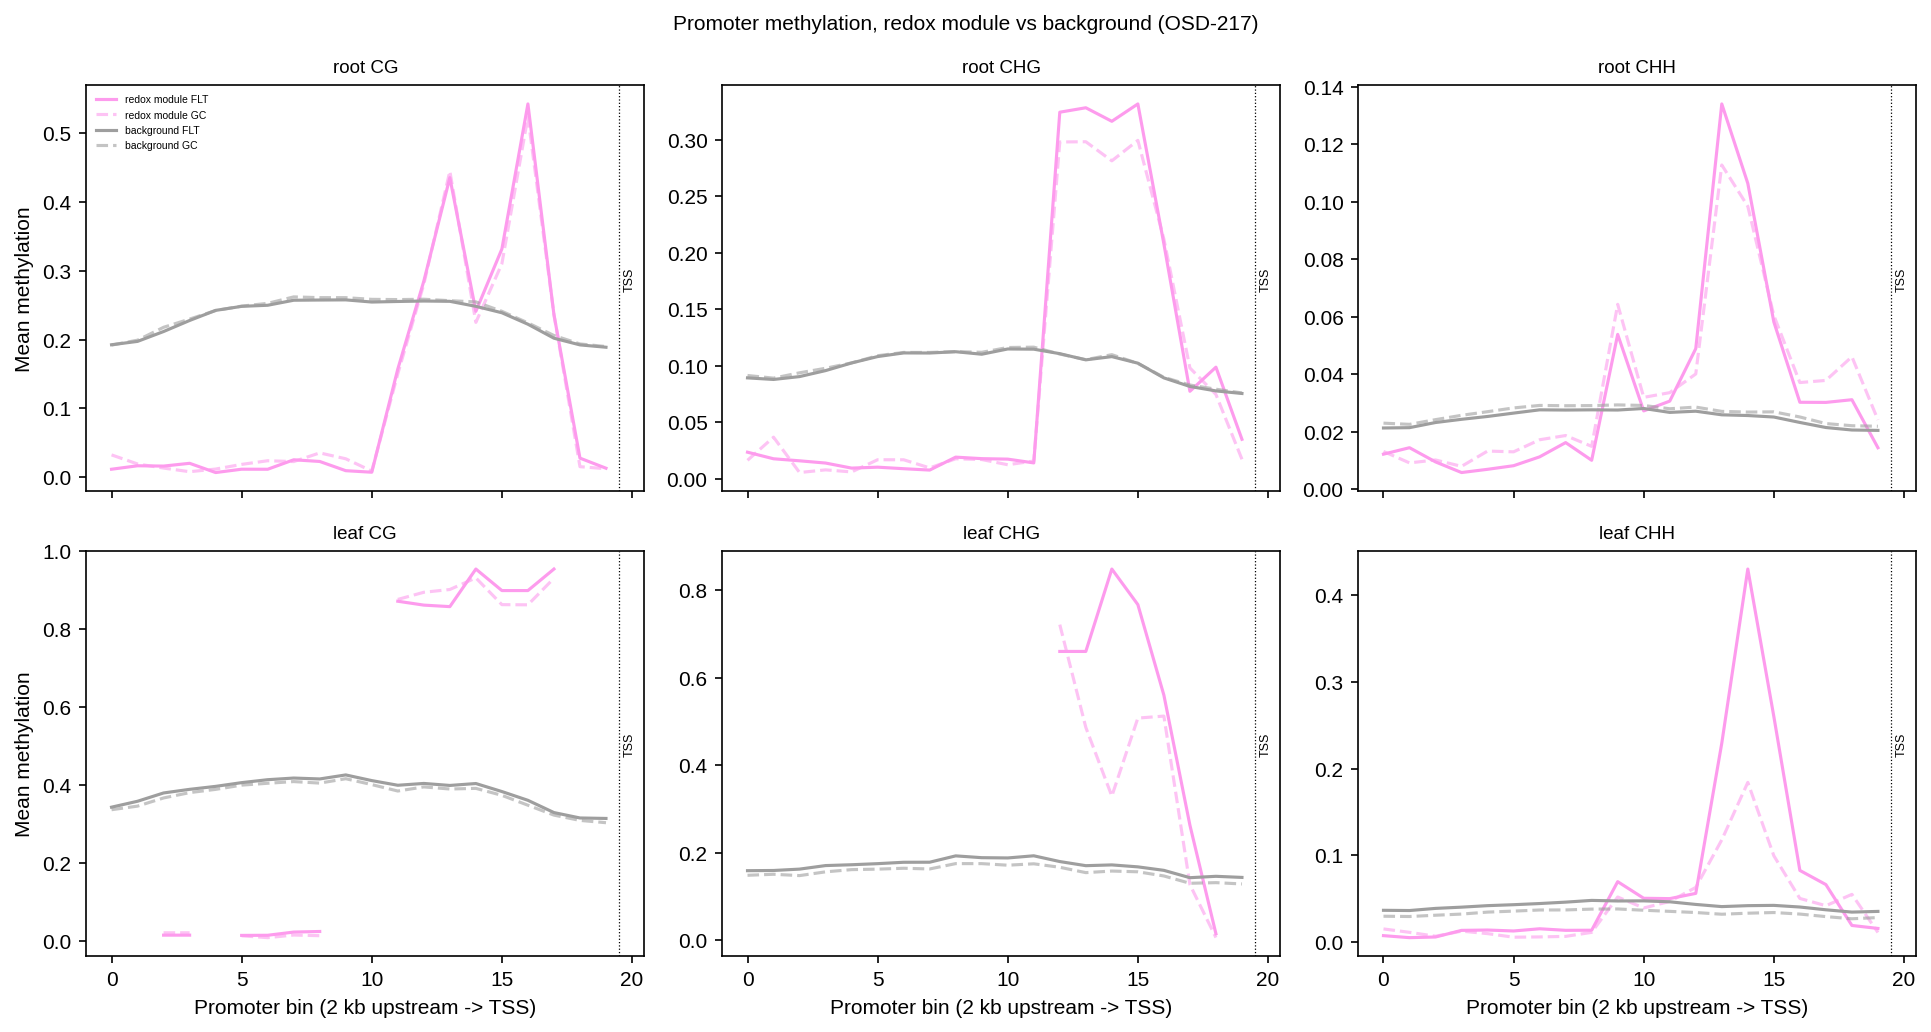
\includegraphics[width=\linewidth]{fig30_promoter_metaplot.png}\caption{}\end{subfigure}
\begin{subfigure}{0.48\textwidth}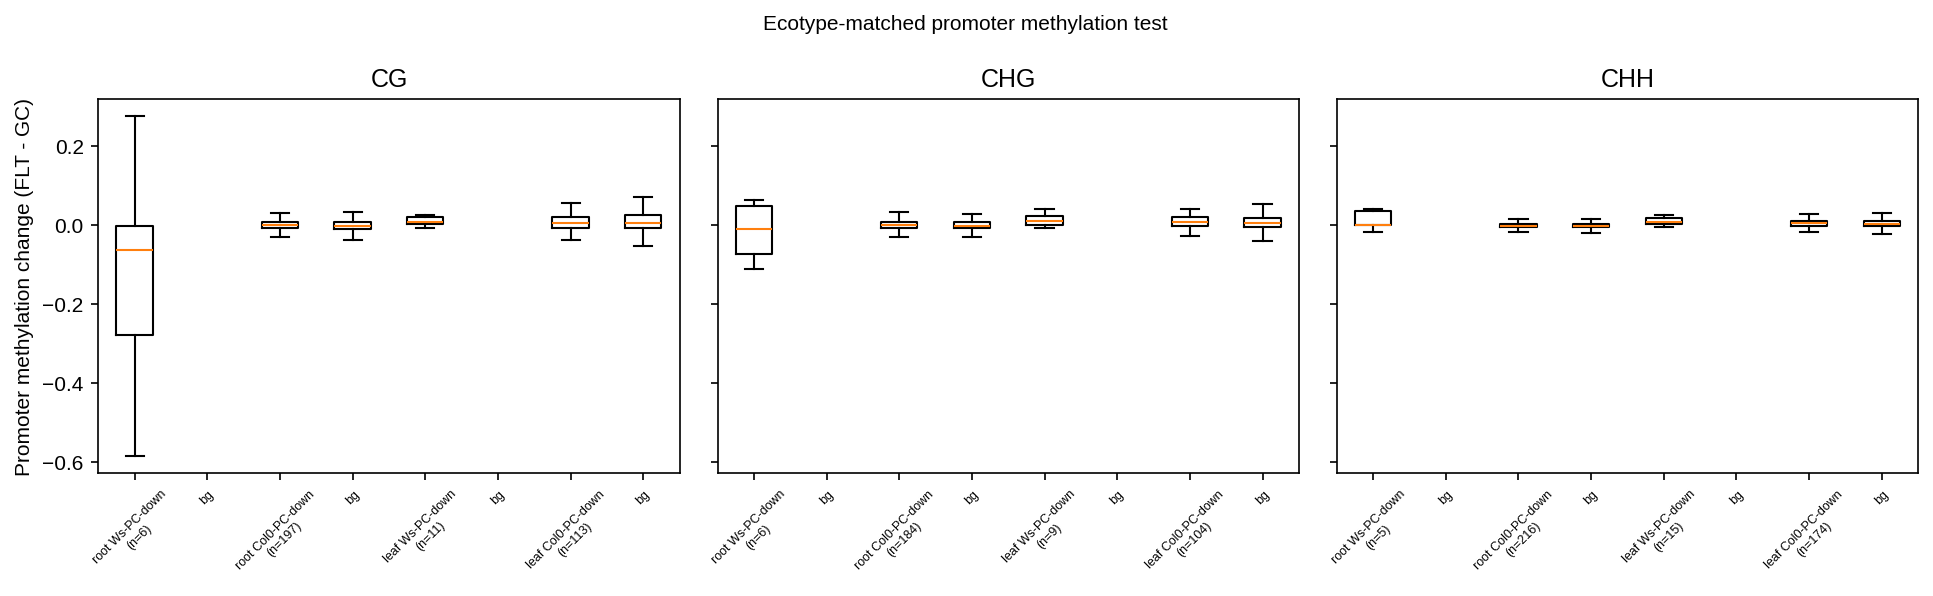
\includegraphics[width=\linewidth]{fig31_ecotype_matched.png}\caption{}\end{subfigure}
\caption{OSD-217 promoter-window methylation (2\,kb, 100-bp bins; Tables~S23--S24). (a) Metaplots by gene set;
leaf coverage is sparse, so the leaf traces are fragmented. (b) Ecotype-matched comparison using the Ws-defined
Polycomb-down module.}\end{figure}

\begin{figure}[h]\centering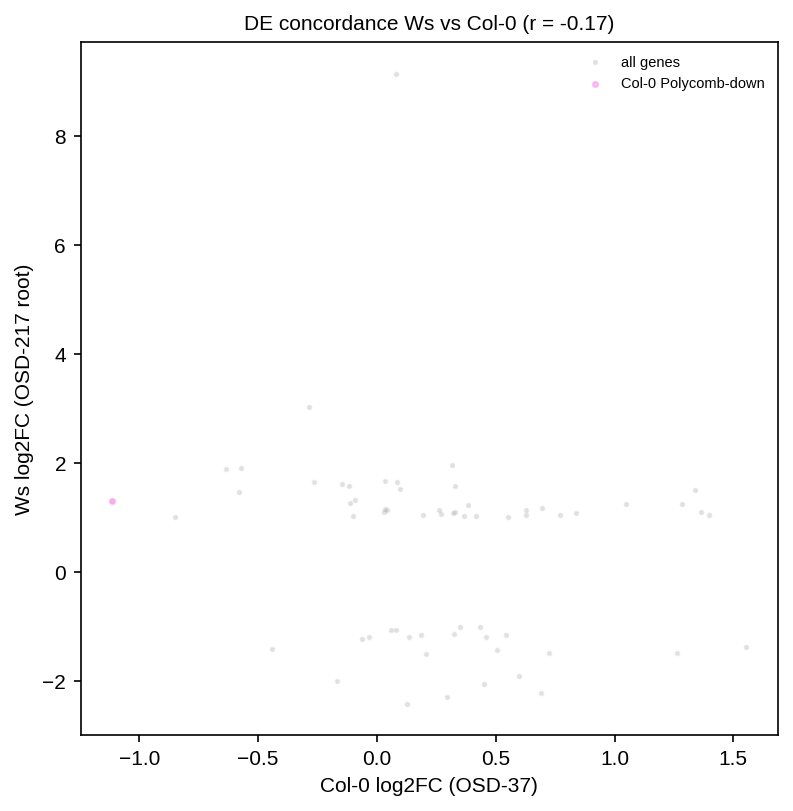
\includegraphics[width=0.55\textwidth]{fig32_ws_col_concordance.png}
\caption{Flight log$_2$FC concordance between OSD-217 (Ws root) and OSD-37 (Col-0 seedlings), $r=-0.17$ over 63
genes (Table~S25).}\end{figure}


\begin{figure}[h]\centering
\begin{subfigure}{0.48\textwidth}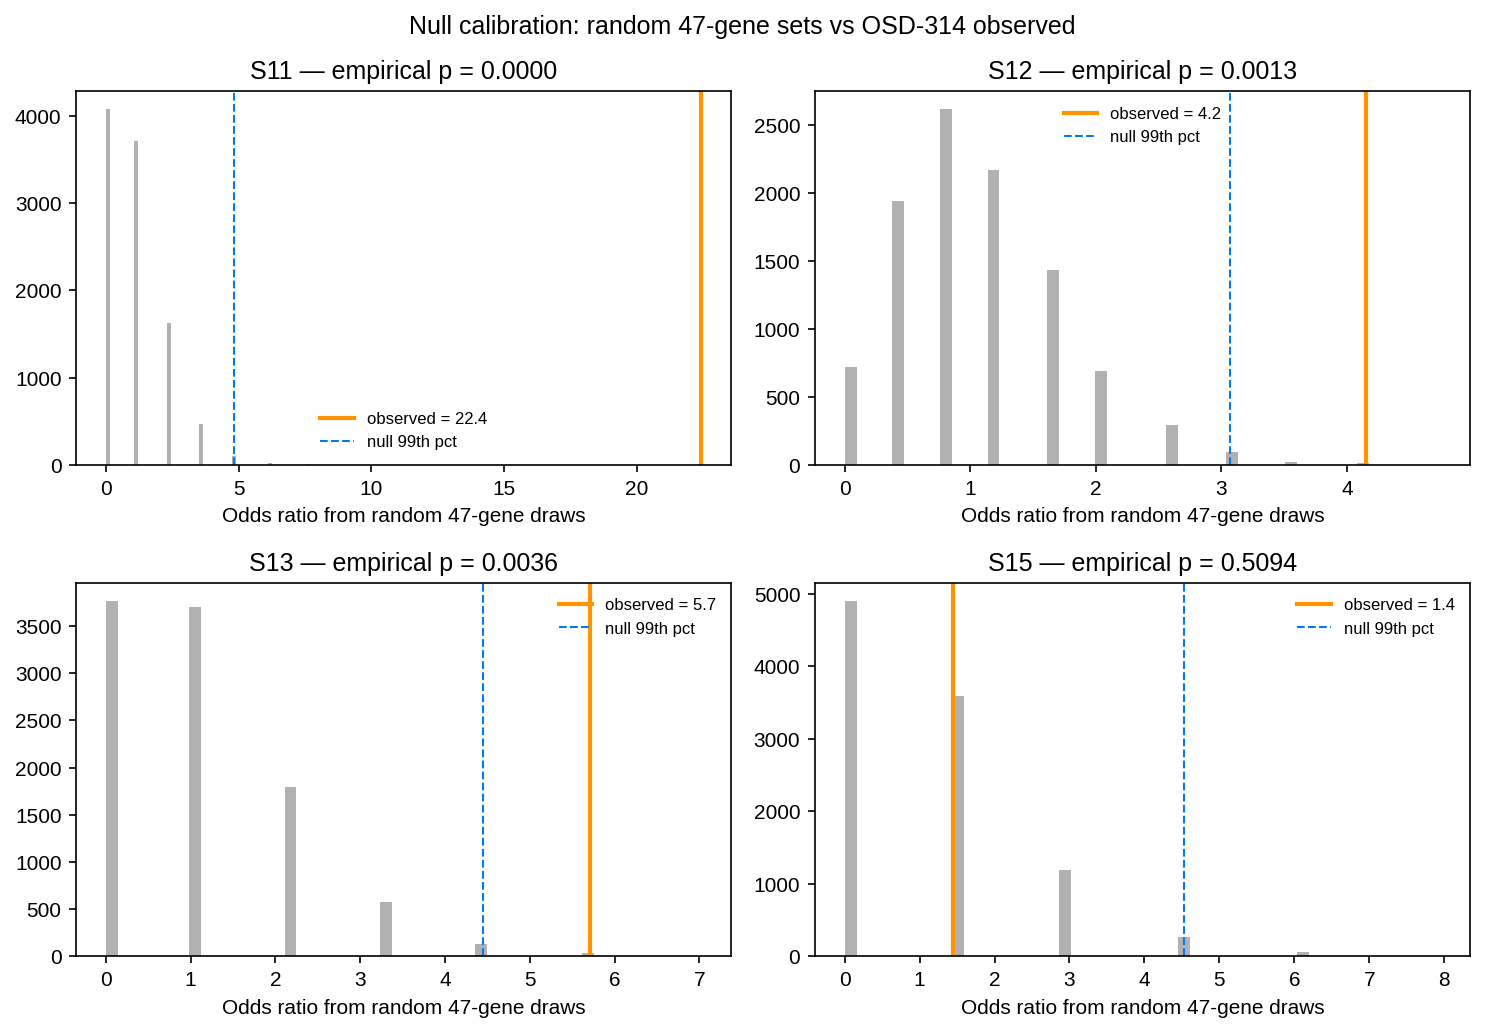
\includegraphics[width=\linewidth]{fig17_null_calibration.png}\caption{}\end{subfigure}
\begin{subfigure}{0.48\textwidth}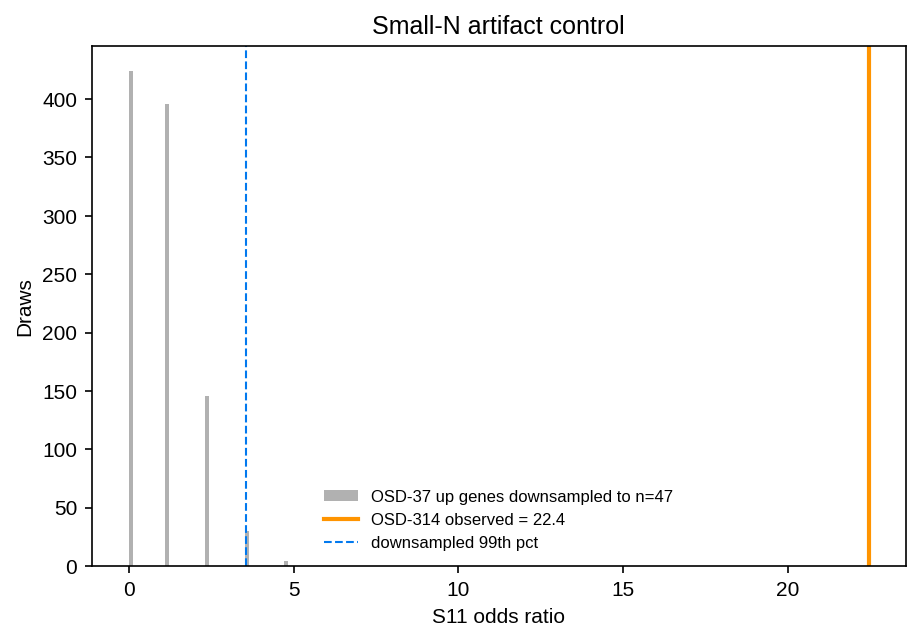
\includegraphics[width=\linewidth]{fig18_downsampling_control.png}\caption{}\end{subfigure}\\
\begin{subfigure}{0.48\textwidth}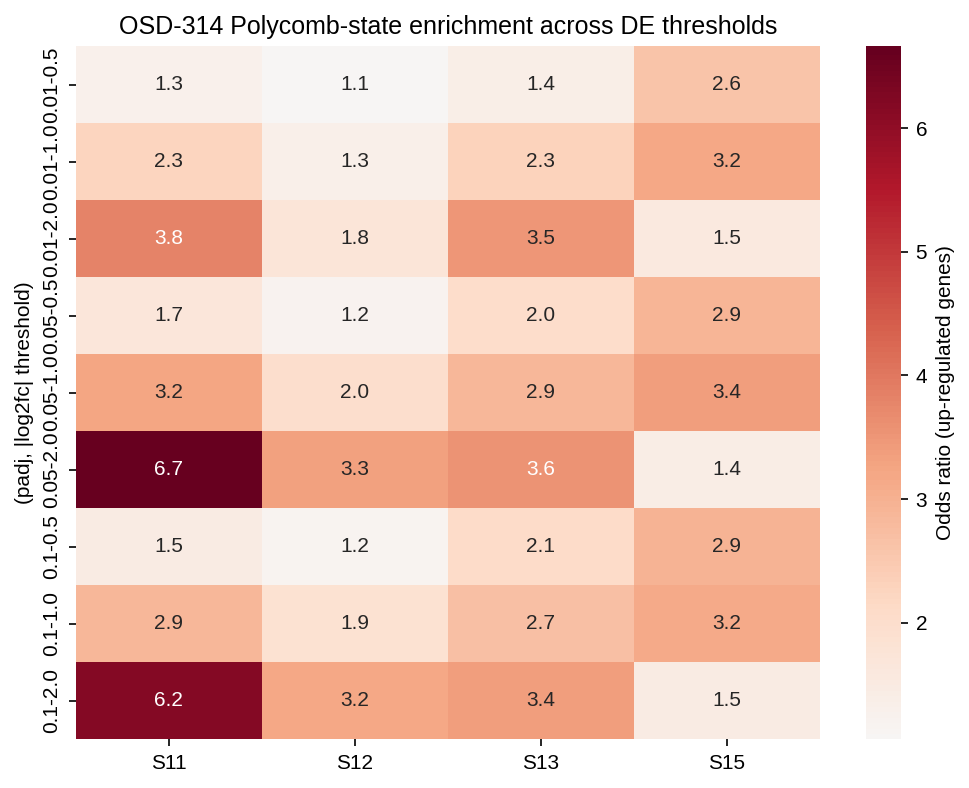
\includegraphics[width=\linewidth]{fig19_threshold_grid.png}\caption{}\end{subfigure}
\begin{subfigure}{0.48\textwidth}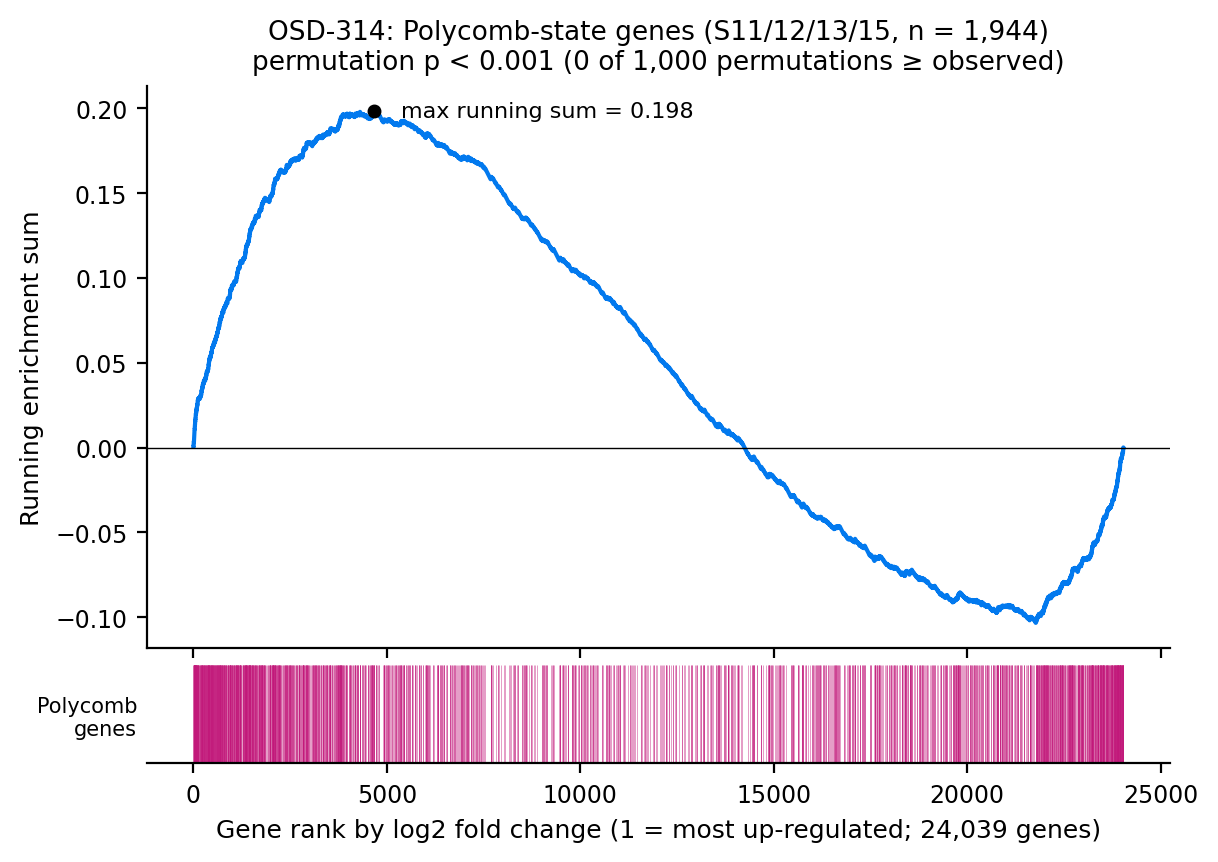
\includegraphics[width=\linewidth]{fig20_running_enrichment.png}\caption{}\end{subfigure}
\caption{Original OSD-314 diagnostics on the published pooled contrast (0\,g + 0.3\,g vs 1\,g; 47 up-regulated genes),
kept for traceability and superseded by main-text Fig.~3. (a) Null calibration (Table~S13). (b) Downsampling control
(Table~S14). (c) Threshold grid (Table~S15). (d) Threshold-free running enrichment (Table~S16).}\end{figure}

\end{document}
